\setstretch{1.6}
\sectiontitle{6}{2D Path following}
\lhead{2D Path following} % section header

\subsection{Background}
\subsubsection{Kinematic Modeling of Similar Devices}
Devices with kinematic similarities to the tendon-driven ribbon-shaped device primarily include steerable needles, concentric tube robots, and tendon-drive continuum robots. Each of these devices rely on structural flexibility and and actuation mechanism that creates a curvature or deformation that allows for navigating through soft biological tissues. Hoever none of them are directly applicable.
\begin{figure} [H]
    \centering
    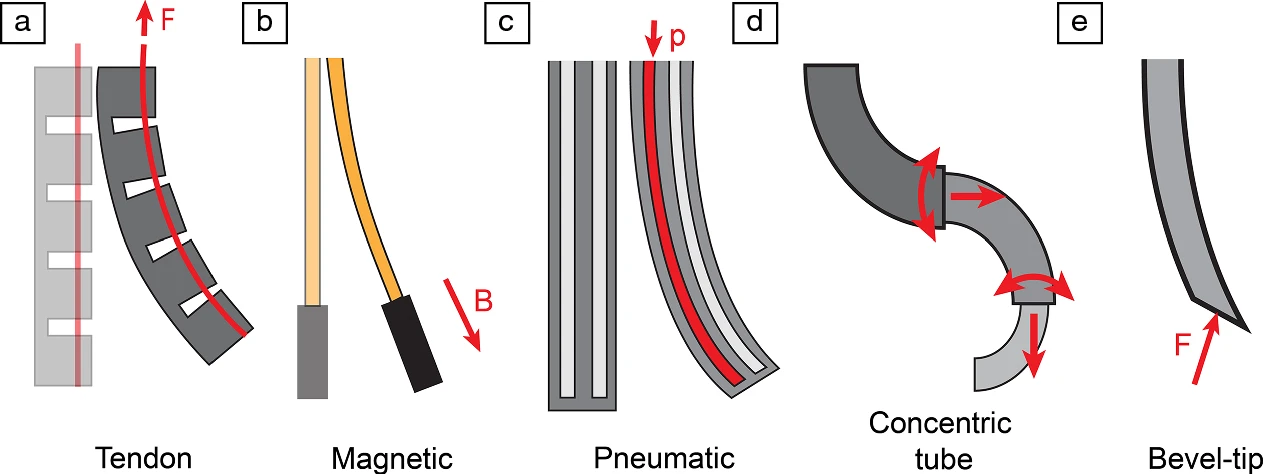
\includegraphics[width=0.9\linewidth]{images/steerableNeedles/actuations.png}
    \caption{Illustration of main actuation and steering mechanisms of small-scale robotic devices developed for brain interventions. Robotic devices can be navigated using (a) tendon-driven mechanisms, (b) magnetic forces and torques, (c) pneumatic systems,  (d) concentric tubes, and (e) slender features with beveled tips. \cite{noseda_small-scale_2024}}
    \label{fig:actuations}
\end{figure}

\paragraph*{Magnetic, Pneumatic and Concentric Tube robots}
Most steerable robotic devices are actuated in a fundementally different manner to the tendon driven ribbon device and must therefore also be steered in a very different way. Magnetic actuation relies on external magnetic fields interacting with embedded magnets \todo{cite}. Pneumatic systems induce curvature by inflating internal chambers which results in a deformation along the entire device  \todo{cite}. Concentric tube robots utilize nested tubes with pre-defined curvatures actuated through relative rotation and translation. Consequently all of these devices kinematics models are not directly transferable to tendon-driven ribbon-shaped devices.

\paragraph*{Traditional tendon-driven continuum robots}
Traditional tendon-driven continuum robots differ significantly to the device used here in their modeling despite their similar actuation. This because they deform continuously along their entire length under actuation forces. While in the ribbon device here it deforms primarily at the distal tip due to the interaction between the backbone and the surrounding brain tissue. Therefore existing continuum robot kinematic models, which assume distributed deformation, cannot be directly applied.

\paragraph*{Steerable Needles}
The device that is by far closest in its steering mechanism are steerable needles, particularly bevel-tip needles. Primarily since steerable needles utilize a deformation at only the tip in order to induce curvature during insertion. This leads to nonholonomic kinematics, meaning the needle's orientation and position are coupled in a way that constrains its possible instantaneous directions of movement i.e. it cannot more laterally without insertion \cite{webster_nonholonomic_2006}. Although steerable needles achieve directional control be rotating the bevel tip or moving segment of the tip as in Secoli et al's work \cite{secoli_adaptive_2016} \cite{secoli_closed-loop_2013}, their steering is still a highly relevant foundation for kinematic models for the tendon-driven ribbon-shaped device.
\newline \newline 
An effective 2D model was developed by Young Ko et al in \cite{ko_two-dimensional_2010}. The steerable probe is modelled as a planar nonholonomic system, where the curvature at the tip determines the trajectory insertion. This curvature is treated as an input to a unicycle-like kinematic model where the evolution of the probe¨s pose is governed by its insertion velocity and current curvature.
\begin{figure} [H]
    \centering
    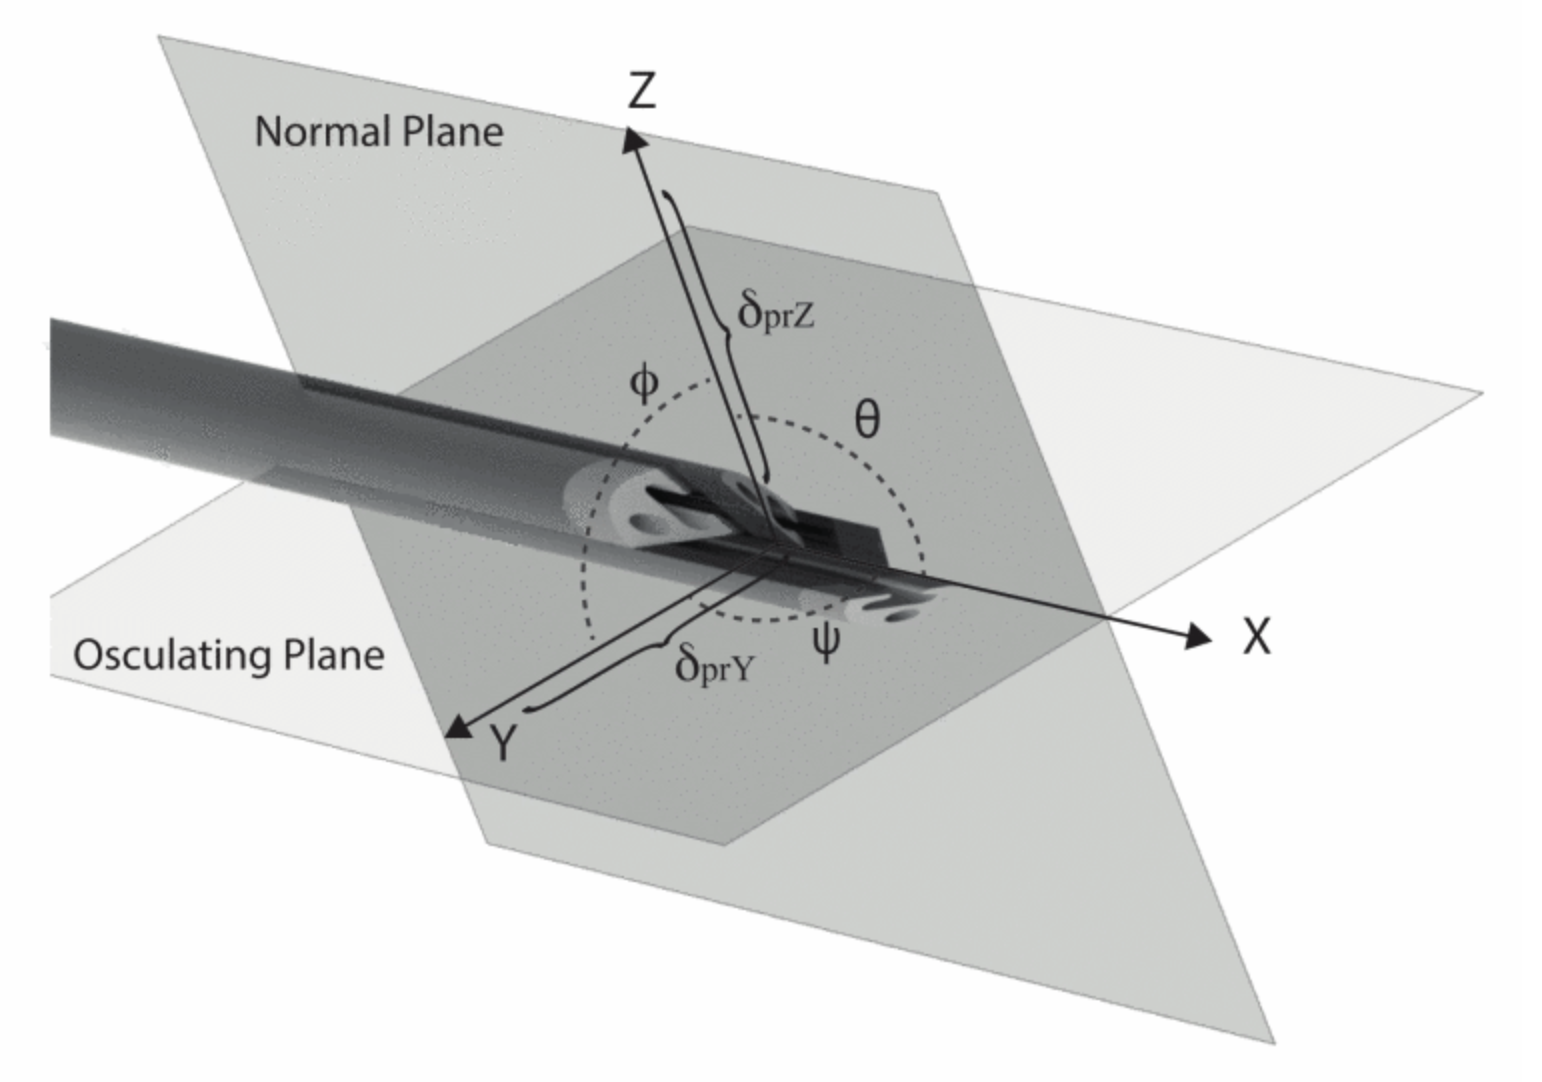
\includegraphics[width=0.7\linewidth]{images/steerableNeedles/needlefig.png}
    \caption{Four part Steerable needle developed by Secoli et al \cite{secoli_closed-loop_2013}}
    \label{fig:fourpartneedle}
\end{figure}
Later Secoli and Rodriguez y Baena developed a 3D version for the same 4-part steerable needle (seen in figure \ref{fig:fourpartneedle}) inspired by underactuated underwater vehicles. The needle's motion is governed by nonholonomic constraints, with insertion along the x-axis and tip steering controlled by programmable offsets between interlocked needle segments. The model defines the needle's orientation using Euler angles (roll, pitch, yaw), with angular velocities about the pitch and yaw axes proportional to the segment offsets. This results in a non-linear, driftless kineamtic system, which they then convert into chained form coordinates for closed-loop feedback control.

\begin{figure}
    \centering
    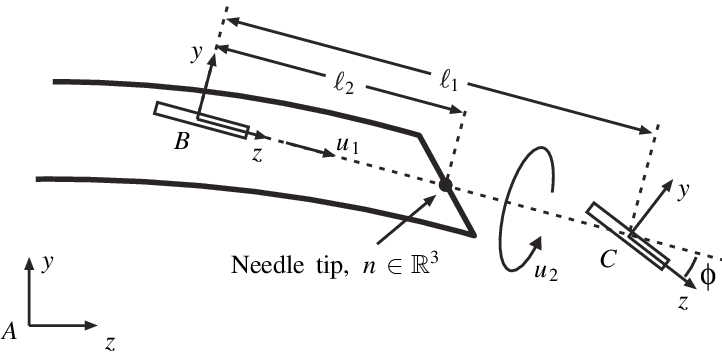
\includegraphics[width=0.7\linewidth]{images/steerableNeedles/Configuration-of-a-bevel-tip-needle-during-steering-showing-the-front-and-back-wheels.png}
    \caption{Configuration of a bevel tipped needle during steering showing the front and back "wheels" \cite{webster_nonholonomic_2006}}
    \label{fig:bicycle}
\end{figure}
A more complex strategy for modeling needle steering is the  model introduced by Webster et al. \cite{webster_nonholonomic_2006}, which treats needle insertion as a constrained control problem similar to a bicycle instead of a unicycle. In bevel-tip needles, the asymmetry at the tip induces lateral forces during insertion naturally creating a curved trajectory where orientation and position are interdependent. For a fixed needle shaft rotation, the model is similar to that of a bicycle with a front wheel angle and a back wheel angle that corresponds to the angle a certain distance from the tip of the needle as is shown in figure \ref{fig:bicycle}.
\newline \newline
Fallahi et al. extended this model for soft tissue and created a model that accounts for non-constant curvature paths for the needle tip. Since for a tissue that is not stiff relative to the needle, the tissue deformation caused by needle insertion deviates the needle tip position. This model is obtained by replacing the bicycle wheels with omnidirectional wheels tha tmove in two orthogonal direction independently. Such wheels can move sideways, providing a means for modeling the deviations of the needle tip from a constant curvature path. \cite{fallahi_extended_2015}



\subsubsection{Path Following Definition}
Path following is a  motion control scenario where a “vessel” has to follow a predefined path without any time constraints \cite{caharija_integral_2016}. It thereby differs to trajectory tracking since the path is not parameterized by time, but rather by another useful parameter \cite{hung_review_2023}, such as path length. 

This distinction is important since in the application to brain surgery spatial control is a lot more critical than timing. Also since the system can make smoother corrections and prioritize accuracy over speed when there are no strict time requirements. Path following also allows smoother convergence to the path and can reduce actuator actuator activity, since it avoids the constant adjustments required by time-based tracking (Aguiar and Hespanha 2007).

\subsubsection{Marine path-following for ribbon navigation in brain tissue}
The steering of the tendon-driven ribbon in brain tissue can be modelled to e kinematacally analogous to that of a boat or UAV. In a marine vessel vessel, turning the helm deflects the rudder, inducin a curvature that realigns the hull with the desired path. In the surgical device, pulling on the tendons causes the flexible tip of the probe to bend in a specific direction. This bending changes the direction of the devices motion, in much the same way that a rudder steers a boat. 
\newline \newline 
Because the bending of the tip of the device directly controls the direction of motion and the relationship between curvature and lateral deviation is governed by the same kinematic principles as in boat steering, the curvature or heading angle computed by marine guiddance laws are directly applicable by converting the heading angle to target bending angle for the device. This target bending angle can then be used to compute the corresponding tendon tensions required to steer the probe along the desired path.
\newline \newline 
Therefore, guidance methods established in marine robotics are well-suited as a foundation for developing the path-following strategy in this application. The following sections therefore provide an overview of the guidance systems popularly employed and developed for marine navigation.

\subsubsection{Types of Guidance systems}
Path following can further be divided into two parts: the guidance system and the control system \cite{qi_curve_2022}. Where the guidance system is responsible for determining the desired target which the control system can then uses in order to steer such that the "vessel" stays on the path, or is lead toward the path if the cross -track error (that is the the shortest distance to the path) is nonzero. Some of the most popular methods adopted by the marine community are line-of-sight(LOS) guidance, pure pursuit guidance, vector field guidance and constant bearing guidance \cite{qi_curve_2022}, \cite{lekkas_integral_2014}. 

\paragraph*{Pure pursuit (Orthogonal Projection)}
In the orthogonal projection/Pure pursuit method the point on path that is closest to the vehicle is used as the "reference point" and then steering towards the point. This leads the along-track error to always be zero and only the corss-track error need to be controlled. The method then computes the desired yaw rate in the case of boaths (i.e. how fast the vehicle should turn) to drive the cross-track error to zero. 
\begin{figure} [H]
    \centering
    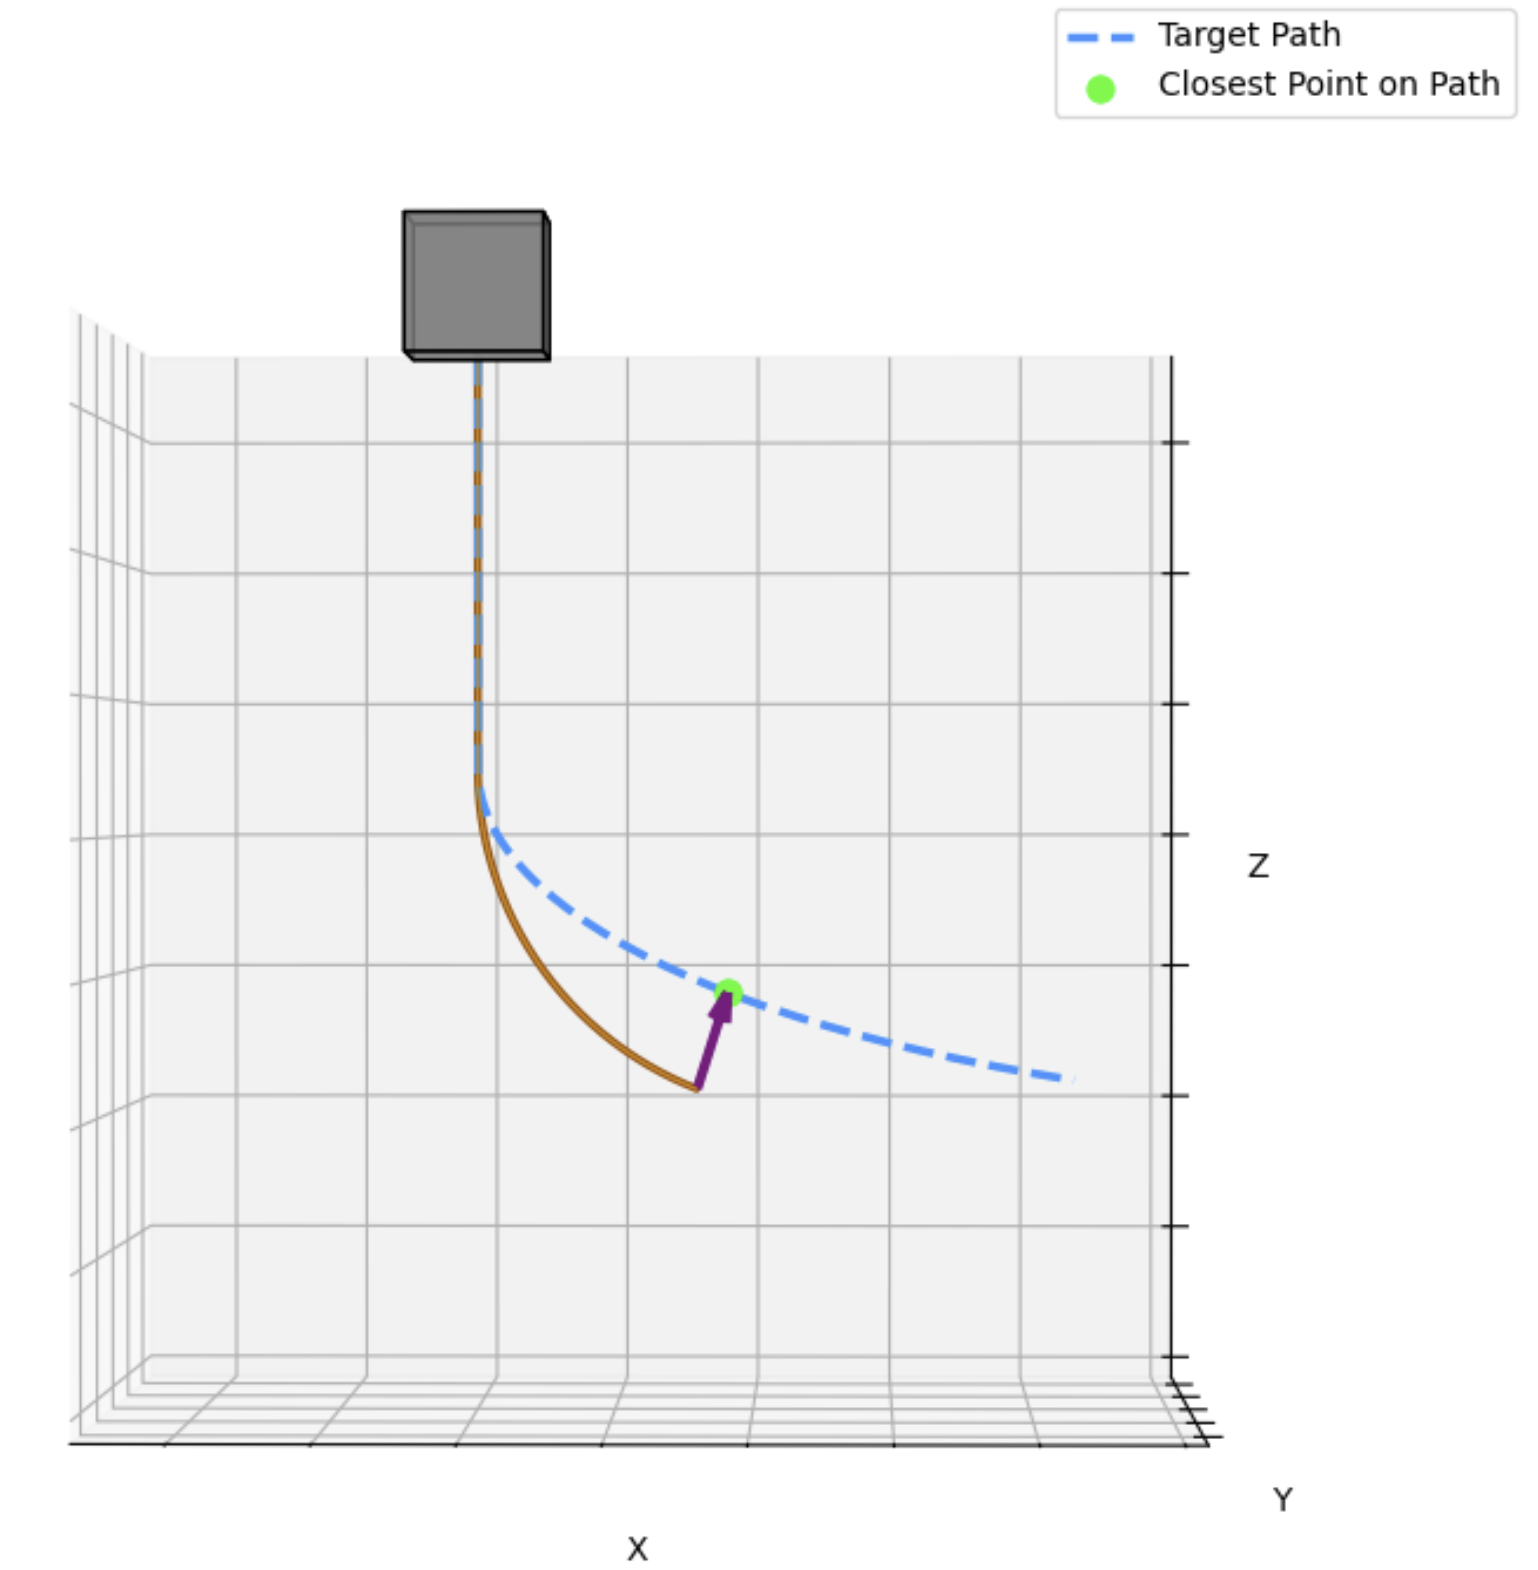
\includegraphics[width=0.7\linewidth]{images/pythonpictures/purepursuit.png}
    \caption{Visualization of orthogonal projection guidance (reference angle being the angle between z-axis and the purple arrow)}
    \label{fig:purepursuit}
\end{figure}
This approach is simple and intuitive. However, the convergence behavior may be problematic in practic. Since the controller always aims for the nearest point on the path it continues to generate turning commands even when the vehicle is nearly aligned. This causes overshooting and unnecessary steering corrections. Further, this method can encounter issues in certain geometric scenarios. Particularly on circular paths when the vehicle crosses the centerpoint of the curvature. In this case the projection onto the path is no longer well-defined and the method can break down.

\paragraph*{Line of Sight}
The LOS guidance method is now widely used due to its small computational cost, easy implementation and intuitiveness \cite{qi_curve_2022} \cite{caharija_integral_2016}. Instead of using the closest point on the path, LOS guidance steers the vehicle toward a point located a fixed distance ahead on the path (known as the lookahead distance). In effect it imitates a helmsman steering the vessel toward a point lying at a constant distance ahead of the ship along the desired path \cite{caharija_integral_2016}. In the case of no enivronmental disturbances, simple LOS has good path convergence properties \cite{borhaug_integral_2008}. 
\begin{figure} [H]
    \centering
    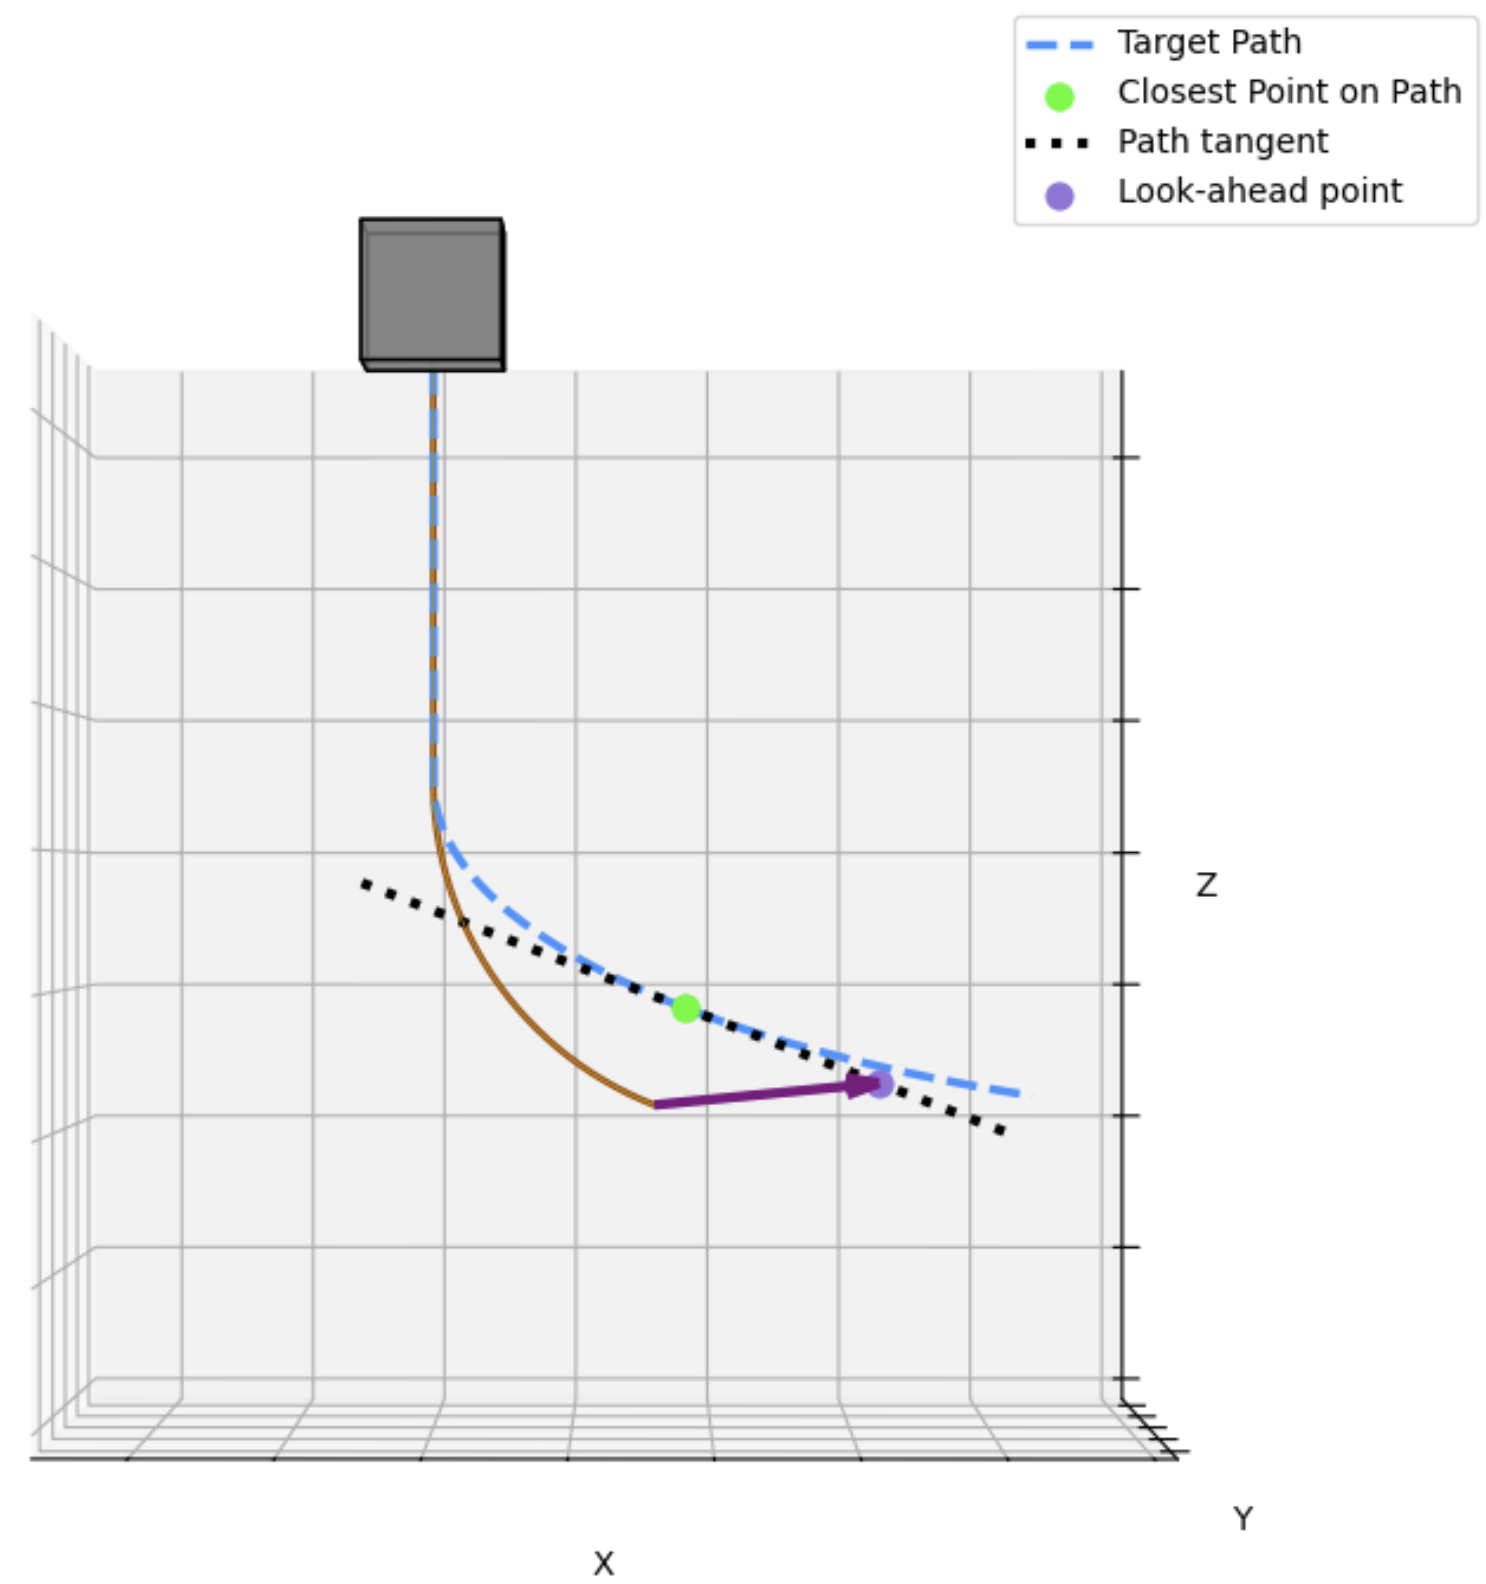
\includegraphics[width=0.7\linewidth]{images/pythonpictures/LOS.png}
    \caption{Visualization of LOS guidance (the angle between the z-axis and the purple arrow becomes the reference pitch angle)}
    \label{fig:LOS}
\end{figure}
However, path following control approaches based on traditional LOS guidance are susceptible to environmental disturbances \cite{borhaug_integral_2008} or more generally all errors that case the actual navigation direction to differ from the guidance direction. In particular this will lead to path deviation and converegence problems \cite{borhaug_integral_2008}. Moreover, this drawback cannot be fixed by simply adding integral action to the heading controller, the problem originates from the heading reference generator, that is, the LOS guidance law itself \cite{borhaug_integral_2008}.

\paragraph*{Integral Line of Sight (ILOS)}
To adress the limitation of traditional LOS, Børghaug et al. \cite{borhaug_integral_2008} proposed a guidance law based on the LOS guidance principle but that includes integral action to overcome the drawbacks of environmental disturbance while preserving the intuition and the simplicity of traditional LOS guidance.
\begin{figure} [H]
    \centering
    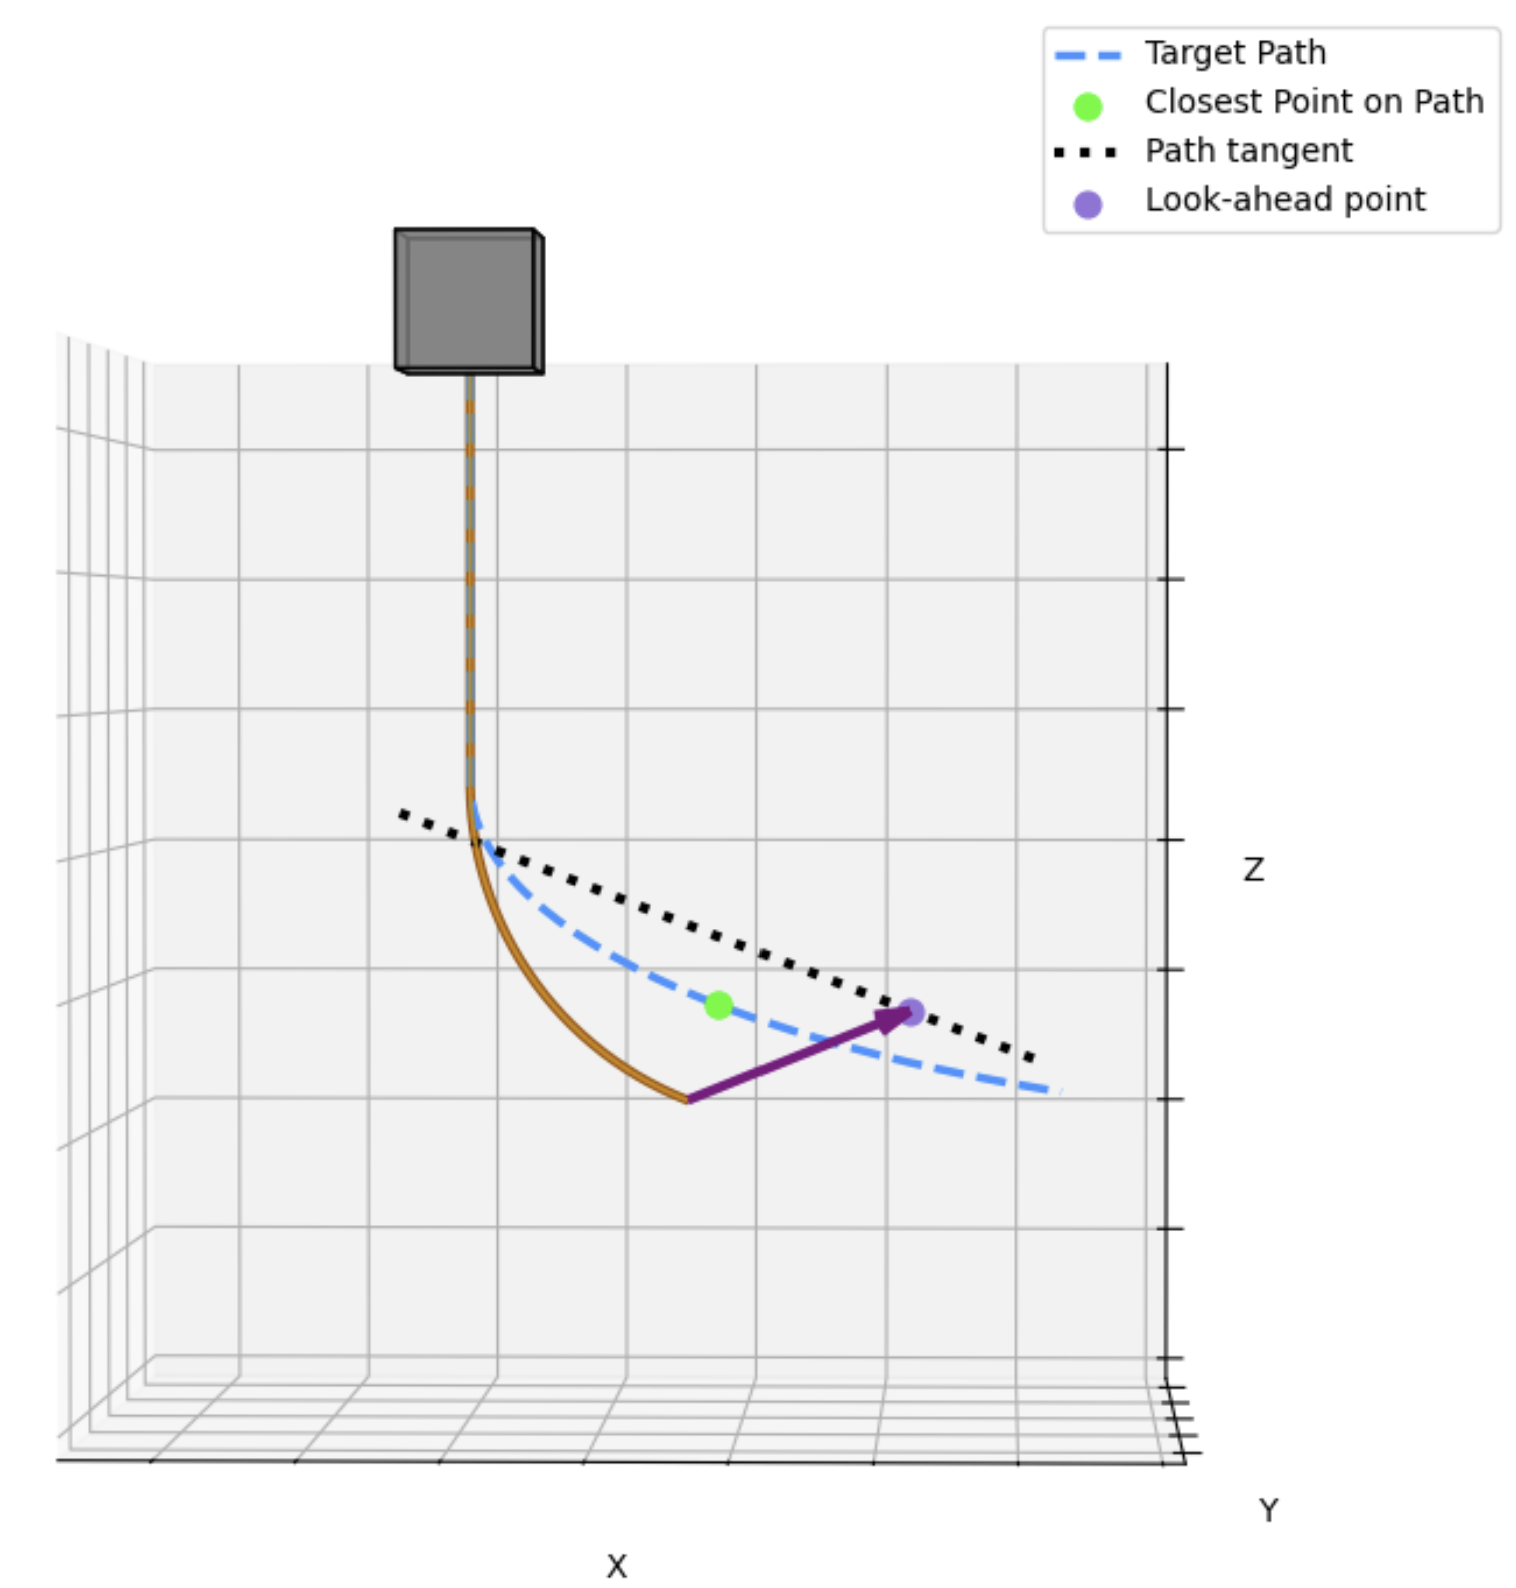
\includegraphics[width=0.7\linewidth]{images/pythonpictures/ILOS.png}
    \caption{Visualization of ILOS guidance (the angle between the z-axis and the purple arrow becomes the reference pitch angle)}
    \label{fig:ILOS}
\end{figure}
By integrating the cross-track error over time, ILOS effectively reduces steady-state error and restores path convergence even when the vessels actual movement direction deviates from its commanded heading.

\paragraph*{Adaptive Methods}
Adaptive guidance methods can improve path-following in uncertain or dynamic environments by adjusting parameters in real time. Several adaptive approaches have been adopted for path-following including adaptive LOS, where the lookahead distance is varied based on cross.track oerror or path curvature \cite{hung_review_2023}. This allows the system to steer more smoothly when far from the path and more precisely when close, reducing overshooting and unnecessary correction.
\newline \newline 
Other methods include adaptive vector field guidance which modifies the synthetic vector field used to steer the vehicle toward the path. By adjusting the shape or strength of the filed based on real-time errors or estimated disturbances \cite{soetanto_adaptive_2003}. Or other techniques including sliding mode control \cite{soetanto_adaptive_2003}, Learning-based MPC and reinforcement learning based control \cite{hung_review_2023}.

\paragraph*{Model Predicitve Control (MPC)}
Model Predictive Control (MPC) is an optimization-based approach that computes control actuation by predicting future system behavior over a finite time horizon. At each time step, it solves and optimal control problem that minimizes path-following error while satisfying system constraints such a speed, turnign limits, and actuator bounds \cite{hung_review_2023}. 
\newline \newline
Unlike geometric methods like LOS or pure pursuit, MPC can explicitly handle physical constraints and nonlinear dynamics. Linear model predictive control, nonlinear MPC and learning-based MPC have all been used in path following research \cite{hung_review_2023}. However they are complicated in terms of design and implementation since they involve solving an optimization problem online. Yet since they deal with the vehicle's input constraints i.e. velocity and angular rate explicitly they are  expected to outperform other path following strategies in cases that require teh vehicle to maneuver more agressively. Another advantage is that they can incoroprate more easily other tasks such as obstacle avoidance in the path following problem. Although using these methods is particularly challenging in environments and with devices that are not easily modeled.





\subsection{Design}

\subsubsection{Choice of Kinematic Modeling Approach}
In the background chapter, several approached previously applied to modeling steerable needles were presented including 2D \cite{ko_two-dimensional_2010} and 3D unicycle models \cite{secoli_closed-loop_2013} as well as bicycle models \cite{webster_nonholonomic_2006} \cite{fallahi_extended_2015}. Based on this review and the physical differences between the ribbon device and the steerable needles a choice was made to begin with a 2D model inspired by the programmable bevel-tip needle work of Ko et al. \cite{ko_two-dimensional_2010}.This model has shown to be effective for steerable needles in soft tissue and its simplicity makes it a good starting off point. If the performance of this method proves insufficient another, more complex model may be adopted later.

\subsubsection{Final 2D Kinematic model}
As mentioned in the hardware section the ribbon device is moved up and down i.e. in the z-plane via control of the linear stage which is attatched at the proximal tip of the device. However movement in the x and y plane is controlled via controlling the tensions at the tendons which are attached to motors at the top and the tip of the ribbon at the bottom. When the ribbon is inserted in a brain phantom via the movement of the linear stage its trajectory will depend on the deflection of the tip. Which is in turn dependent on the tendon activation pattern which results in the bending or twisting of the tip. 
\newline \newline
To capture this behavior a unicycle type model inspired by \cite{ko_two-dimensional_2010} is used where the tip orientation is described using an Euler angle representation, which describes the orientation between the global frane and the local body coordinate frame as three rotations: roll \(\\phi\), pitch \(\theta\) and yaw \(\psi\) which represent rotations about the local body cartesian axes \(x\), \(y\) and \(z\) respectively.

\begin{figure} [H]
    \centering
    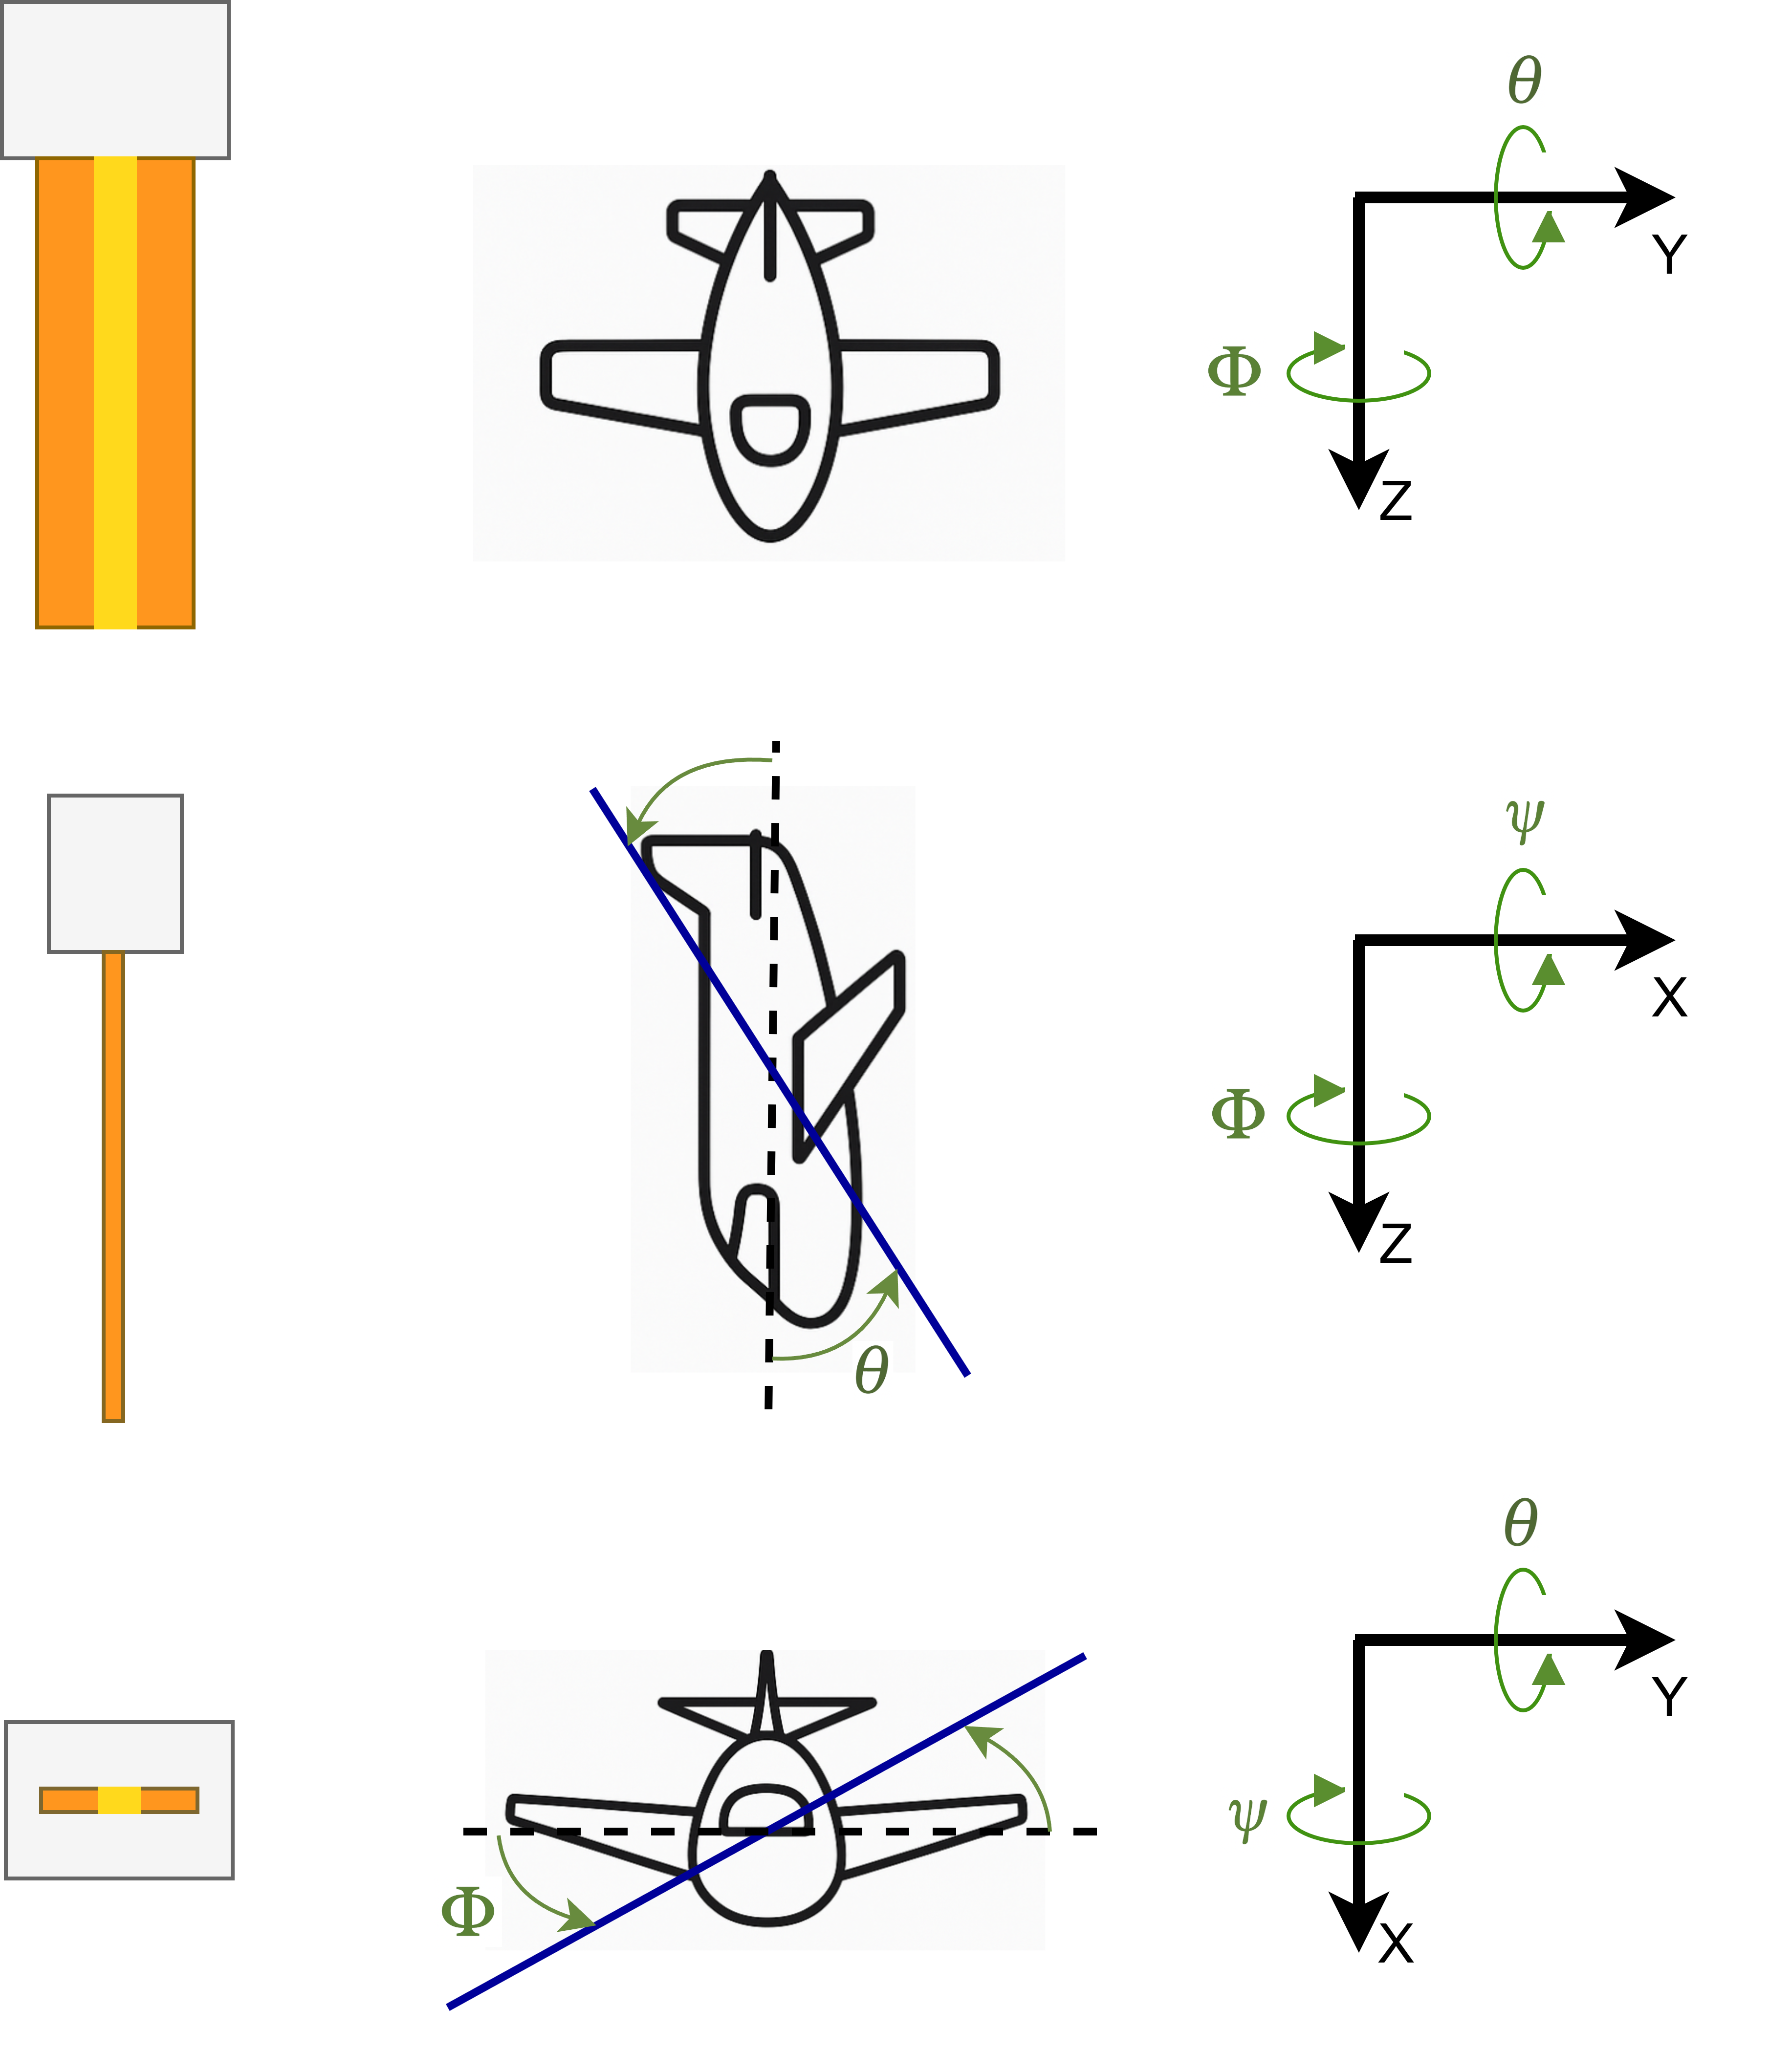
\includegraphics[width=0.7\linewidth]{images/planes.png}
    \caption{Visualization of the definition of Euler angles for the ribbon system and its analogy to vehicle models}
    \label{fig:planes}
\end{figure}


\begin{figure} [H]
    \centering
    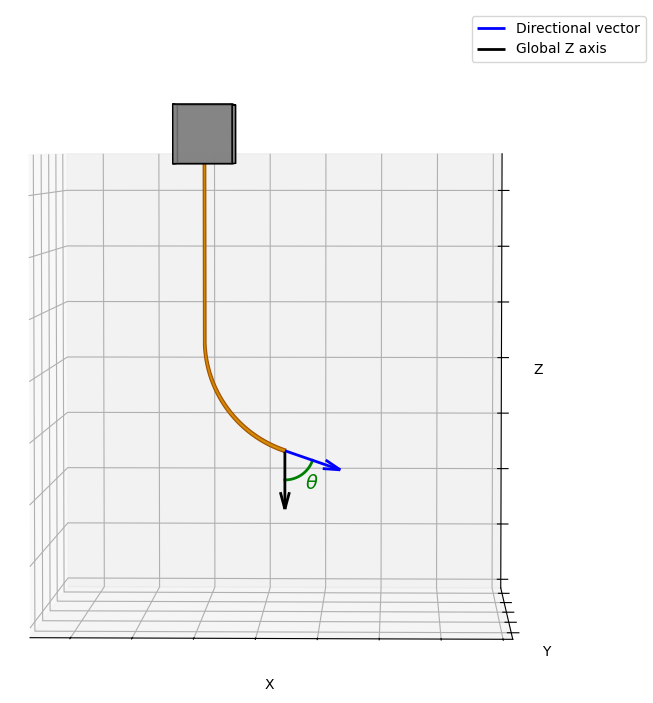
\includegraphics[width=0.55\linewidth]{images/pythonpictures/Capture.PNG}
    \caption{Visualization of the $\theta$ angle the determines the rotation around the local y-axis}
    \label{fig:theta}
\end{figure}

In the 2D kinematic model we assume the global y-position to be constant and thus there is no velocity component along that axis. When the tip bends in order to follow a trajectory it is performing a rotation around the local y-axis in the x-z-plane as is visualized in figure \ref{fig:theta} and \ref{fig:planes}. The rotational matrix thereby becomes

\begin{equation}
    \textbf{R} = \textbf{R}(\theta) = \begin{bmatrix}
        cos \theta   &   0   &   -sin \theta \\
        0            &   1   &   0\\
        sin \theta   &   0   &   cos \theta
    \end{bmatrix}
\end{equation}
and the kinematic model becomes
\begin{equation}
    \vec{v_g} = \textbf{R}(\theta) \vec{v_b}
\end{equation}
Where $\vec{v_g}$ signifies the velocity of the tip in the global frame, \textbf{R}$\theta$ is the rotational matrix around the y-axis that transforms the body velocity of the tip of the ribbon given in the body frame $\vec{v_b}$ to the global frame. Inserting the previously defined rotational matrix we have:
\begin{equation}
    \begin{bmatrix}
        \dot{x}\\ \dot{y}\\ \dot{z}
    \end{bmatrix} = 
    \begin{bmatrix}
        cos \theta   &   0   &   -sin \theta \\
        0            &   1   &   0\\
       -sin \theta   &   0   &   cos \theta
    \end{bmatrix}
    \begin{bmatrix}
        v_x^b \\ v_y^b \\ v_z^b
    \end{bmatrix}
\end{equation}

\begin{equation}
    \begin{bmatrix}
        \dot{x}\\ \dot{y}\\ \dot{z}
    \end{bmatrix} = \begin{bmatrix}
        v_x^bcos \theta - v_z^b sin \theta\\
        v_y^b\\
        v_x^b sin \theta  v_z^b cos \theta
    \end{bmatrix}
\end{equation}
However since we are in the 2D case where \(v_y^b = 0\) we can simplify this to:
\begin{equation}
        \begin{bmatrix}
        \dot{x}\\ \dot{z}
    \end{bmatrix} = \begin{bmatrix}
        v_x^bcos \theta - v_z^b sin \theta\\
        v_x^b sin \theta + v_z^b cos \theta
    \end{bmatrix}
\end{equation}
Further since the ribbon is inserted via the linear stage moving the backbone down the velocity along the ribbons z-axis will be the only significant velocity component in a stiff medium, therefore we can further simplify the model to.
\begin{equation}
	\begin{bmatrix}
	\dot{x} \\ \dot{z}
	\end{bmatrix} = \begin{bmatrix}
	-sin\theta \\ cos\theta
	\end{bmatrix} v_z^b
\end{equation}

In terms of the rotational velocity, it is defined by the relationship between the instantaneous curvature $\kappa$ at the tip and the insertion velocity $v_z^b$. Since 
\begin{equation}
    \frac{d}{dt}\theta  = \frac{d\theta}{ds}\frac{ds}{dt}=\kappa v_z^b
\end{equation}

\begin{figure} [H]
    \centering
    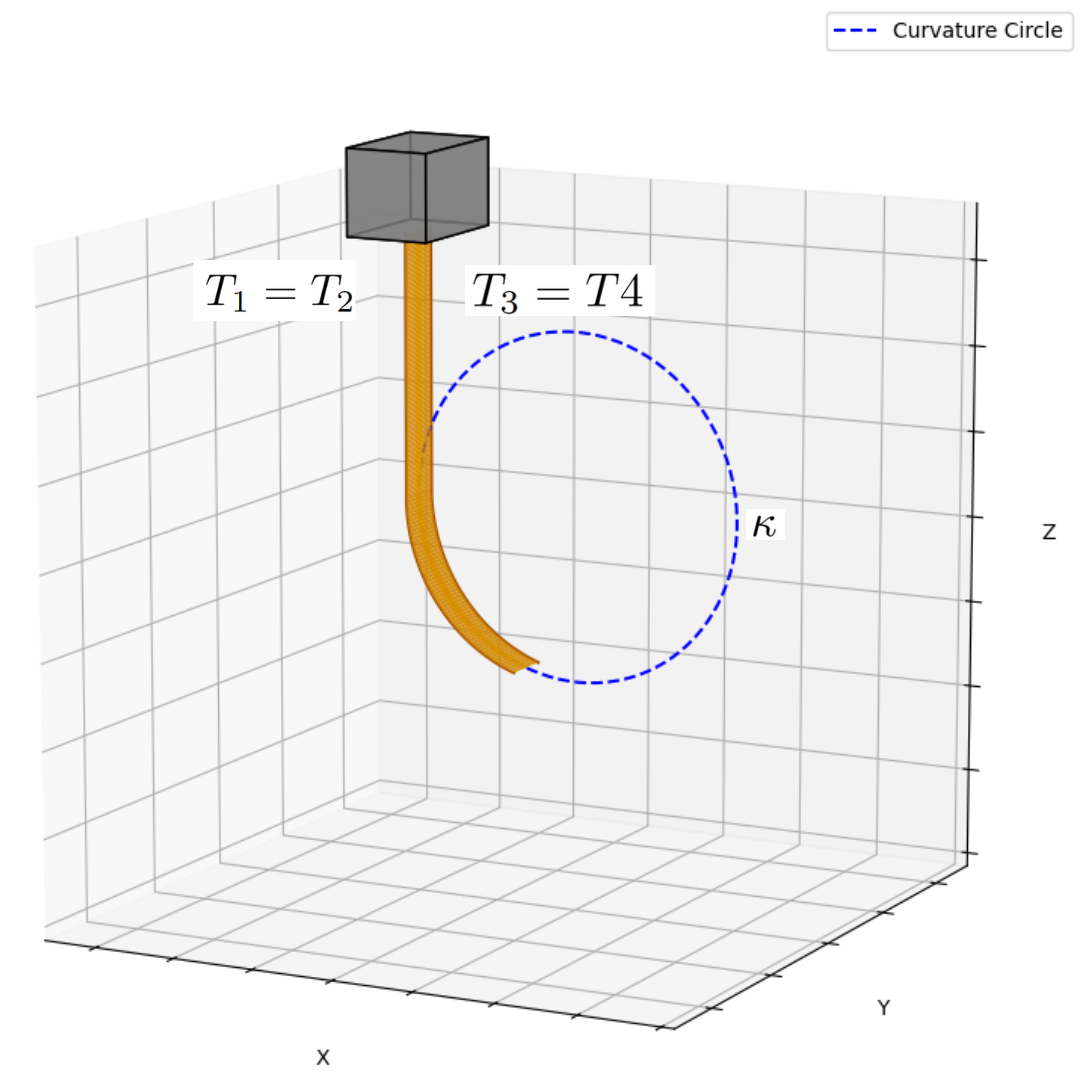
\includegraphics[width=0.6\linewidth]{images/pythonpictures/curvature.PNG}
    \caption{Visualization of how the curvature of the tip $\kappa$ controlled by the difference in tension on the left side \(T_1, T_2\) and right \(T_3, T_4\) influences the trajectory of the ribbon}
    \label{fig:curvature}
\end{figure}

The instantaneous curvature $\kappa_{tip}$, visualized in figure \ref{fig:curvature} is further assumed to be a function of the difference in tension between the tendons on the right and left side $f(u)$, which is given by the actuation variable defined as $u$. Where $f(u)$ is a monotonically increasing function of the actuation variable. In this project this is simplified to be a linear function, independent of previous states and defined by only the offset $b$ and the slope $a$. 
\begin{equation}
	\kappa_{tip} = f(u) = a\cdot u + b
\end{equation}

Including the angular velocity in the system model we arrive at the final 2D model:
\begin{equation}
	\begin{bmatrix}
		\dot{x} \\ \dot{z} \\ \dot{\theta}
	\end{bmatrix} = \begin{bmatrix}
	-sin\theta \\ cos\theta \\ f(u)
	\end{bmatrix}v_z^b
\end{equation}



\subsubsection{Final 2D Control System Design}

\begin{figure} [H]
    \centering
    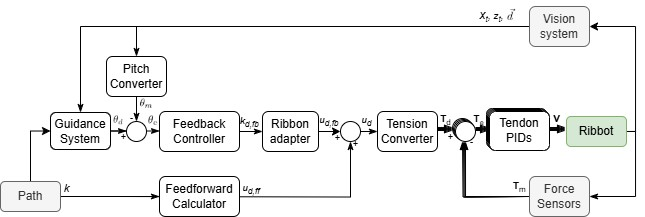
\includegraphics[width=\linewidth]{images/RibbotControl_V2.png}
    \caption{Full control system diagram for 2D path following}
    \label{fig:2Dcontrol}
\end{figure}
A visualization of the full control system architecture for 2D path following is shown in figure \ref{fig:2Dcontrol}. The system uses a predefined spatial path as reference (see Path Planning Integration chapter) and continuously adjusts the tendon tensions to steer the ribbon tip along this path. The current position \((x_t, z_t)\) is extracted from vision data (see Tip Tracking Integration chapter) and passed to the \texttt{GuidanceSystem}, which computes the desired pitch angle \(\theta_d\). The orientation of the tip \(\vec{d}\) is also extracted from the vision data and passed to the \texttt{PitchConverter} which calculates the measure pitch angle \(\theta_m\). The desired pitch angle \(\theta_d\) is then compared to the measured pitch angle \(\theta_m\), and the resulting error \(\theta_e\) is used by the feedback controller, here a PI controller to compute a corrective curvature command \(\kappa_{d,fb}\) which in this system corresponds to how fast the pitch changes as the ribbon advances in space since 
\begin{equation}
    \kappa = \frac{d\theta}{ds}
\end{equation}
Before any path following is done the ribbon is run through a calibration protocol where its bending dynamics based on tendon tension are mapped, after this has been mapped the user inputs this into the gui and the \texttt{RibbonAdapter} module that receives the desired corrective \(\kappa_{d, fb}\) uses this in order to calculate the appropriate actuation value \(u_{d, fb}\) in order to achieve the desired curvature for this particular ribbon. The actuation value \(u\) is defined as 
\begin{equation}
    u = T_{3,4} - T_ {1,2}
\end{equation}
Where \(T_{3,4}\) corresponds to the tension on tendon 3 and 4 which are placed on the right side, and \(T_{1,2}\) corresponds to the tension on tendon 1 and 2 which are on the left side. 
\newline \newline
To assist the controller and improve responsiveness, a feedforward signal based on the local path curvature at the closest point is calculated by the \texttt{FeedbackCalculator} modulate. This feedbackterm \(u_{d, ff}\) is then combined with the feedback term and sent to the \texttt{TensionConverter} module. This module converts that actuation value into individual tendon tension targets \(\textbf{T}_d\) based on a set of rules which ensure a baseline tension is maintained and tension limits aren't exceeded. These targets are then sent to the low-level tension controllers (see closed-loop tension control chapter) which ensure that the tendons track their tension targets using feedback from force sensors.
\newline \newline
This modular and layered control structure supports accurate and smooth path following, while being modular and scalable. 


\subsubsection{Choice of Guidance system}
The chosen path-following strategy must above all be reliable, modular and suit the constraints of the ribbon-based system. Among the available options, pure pursuit, LOS, ILOS, adaptive and MPC, the initial chosen strategy is LOS guidance is it is a simple yet very effective solution to path following.
\newline \newline 
Although more advanced techniques such as MPC or more advanced form of adaptive control could provide better performance in theory, they are currently impractical for this system. In particular, implementing MPC poses siggnificant challenges because of teh highly nonlinear and complex dynamics of the ribbon. The tendon actuation results in strong coupling between degrees of freedom and the deformation fo the ribbon is influenced by wear, material hysteresis, bucklin and loading history. The future surgical environment adds another layer of complexity through contact forces with tissue that are difficult to predict and incorporate into the optimization framework. All of which make it extremely difficult to develop an accurate predictive model required for MPC.
\newline \newline
For these reasons, LOS offers a better, more practical solution. LOS is relatively straightforward to implement and has good convergence properties in undisturbed environments. It is also very easy to expand upon by adding a integral term, creating a ILOS guidance system that would better handle disturbances. It can even be made adaptive by making the look-ahead distance change based on chosen factors. It is therefore a good starting off point for the system.

\subsubsection{Final LOS Guidance System Design}

\begin{figure} [H]
    \centering
    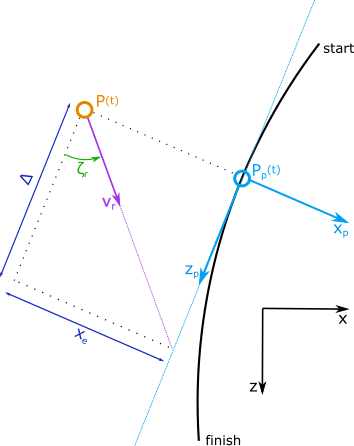
\includegraphics[width=0.6\linewidth]{images/inkscape/pathframe.png}
    \caption{Caption}
    \label{fig:enter-label}
\end{figure}



\subsection{Methods}

\subsubsection{Path-Following Implementation Methodology}
In order to ensure that later expansions or improvements to the 2D path-following would be easy to implement and the system be highly readable the  system is implemented using a modular architecture that consists of a \texttt{GuidanceSystem}, \texttt{PitchConverter}, \texttt{FeedbackController}, \texttt{FeedforwardCalculator}, \texttt{RibbonAdapter} and \texttt{TensionConverter}. These modules correspond to classes in the code base inside the pathfollowing folder and correspond directly to the modules in the control system diagram as can be seen in figure \ref{fig:2DpathfollowingSystemControlDiag}. 

\begin{figure} [H]
    \centering
    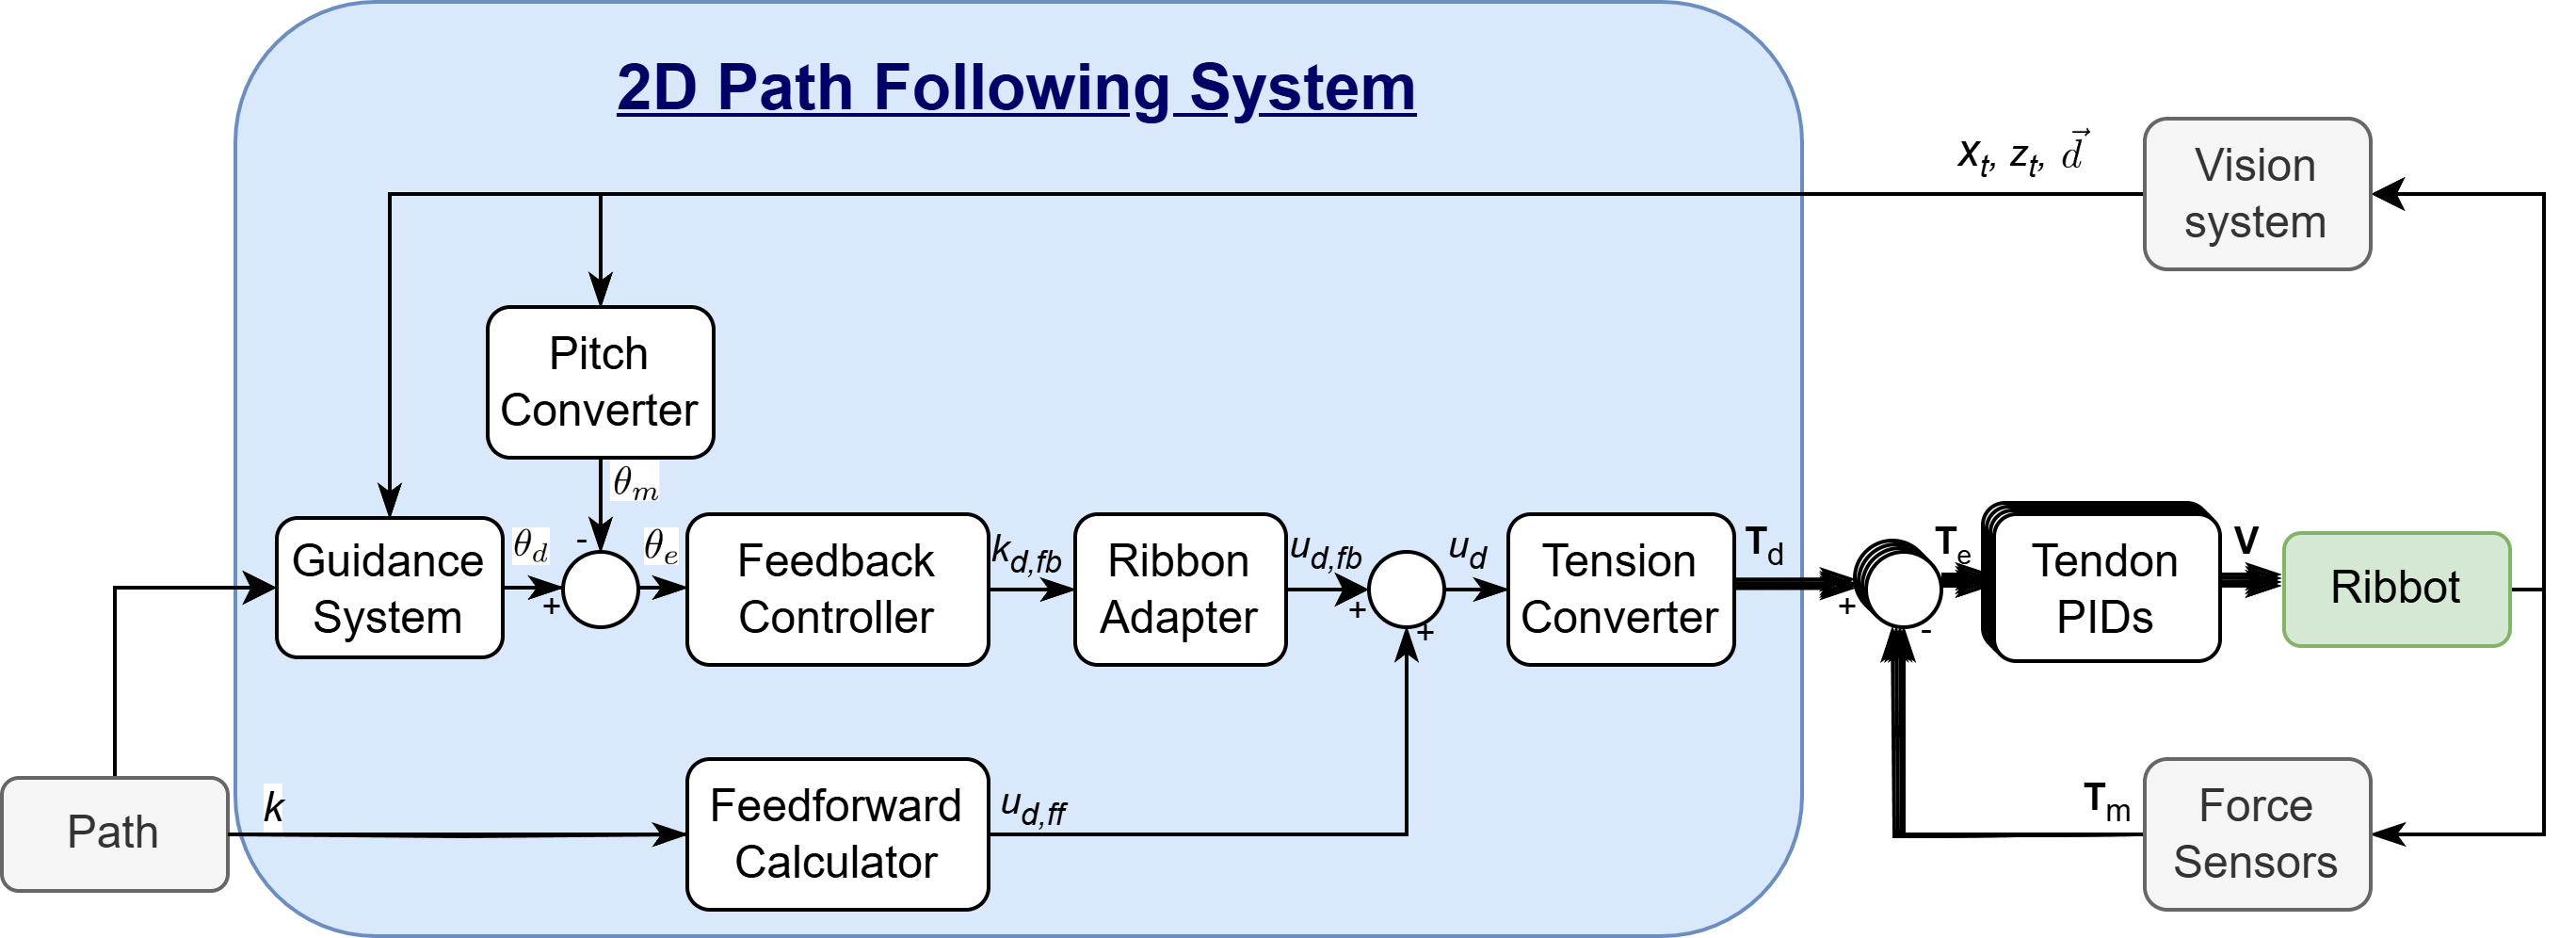
\includegraphics[width=\linewidth]{images/RibbotControl_2Dpathfollowing400p.png}
    \caption{Visualization of the 2D path following system section of the full control system}
    \label{fig:2DpathfollowingSystemControlDiag}
\end{figure}

In order to orchestrate the cooperation between these classes and their dataflow the \texttt{PathFollower} class was created. This class is also responsible for communicating with the rest of the code base. Its connection to the other classes can be seen in figure \ref{fig:pathfolloingmodules}.   In the later chapter on implementation each of the modules are expanded upon and explained.

\begin{figure}[H]
    \centering
    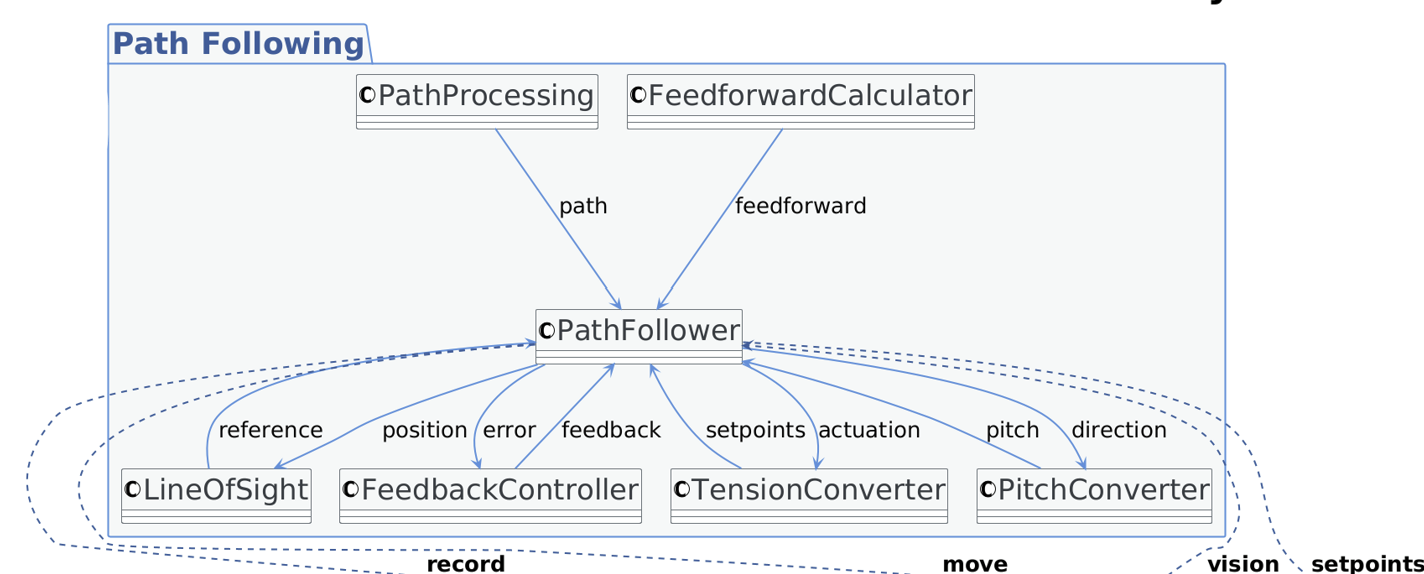
\includegraphics[width=\linewidth]{images/Software documentation/pathfollowingmodules.png}
    \caption{Path following system architecture}
    \label{fig:pathfolloingmodules}
\end{figure}



\paragraph*{Guidance}
The \texttt{Guidance} class implements the core navigation algorithm that generates heading references based on the current tip position and the desired path.

\paragraph*{title}

\subsubsection{Pitch autopilot}
In order for the ribbon to follow the path, the tip must continuously align wiht the desired pitch angle \(\theta_{ref}\) computed by the lOS algorithm. However,the physical system is controlled through tendon tensions which induce bending at the distal tip. Therefore, an intermedediate control layer, a pitch autopilot, must be implemented to convert heading references into actuator-level commands.
\newline \newline
It was decided 

\subsubsection{Tuning}
the Ziegler-Nichols relay method assumes that:

The system has an oscillatory behavior when switching between min and max control effort.

The output returns toward the setpoint (or crosses it) once actuation is disabled, creating that nice sine-like signal from which to estimate the ultimate gain and period.

But in your case — tendon-actuated heading control — that doesn’t apply:

Once you've pulled the tendons to deform the tip and achieve a certain heading, the heading stays there unless you actively pull the other way.

There’s no natural restoring force — no spring-back, no drift back — so the "relay" logic of toggling output and watching the system cross the setpoint repeatedly breaks down.

This is more like trying to autotune a position-controlled robot arm joint where gravity and friction dominate and the joint stays where it's told.

\subsubsection{Validation of Path Following}


\subsection{Implementation}

\subsubsection{Guidance System (LOS)}


\subsubsection{Pitch autopilot}
The pitch autopilot is a closed-loop control system that continuously regulates the pitch of the tip. The autopilot layer consists of three primary components: a pitch angle converter, a feedback controller, and a tension converter. Together, these components transform the LOS heading reference into actuator-level tendon tension setpoints.

\subsubsection{Pitch converter}
The first step in the autopilot is estimating the measured pitch angle, \(\theta_{meas}\), from vision data. This is simply done by computing the angle between the z-axis and the 3D direction vector defined by the detected tip and pre-tip positions. 
\begin{equation}
    \theta_{meas} = atan2(\vec{d}_x,\vec{d}_z)
\end{equation}
where \(\vec{d}_x\) and \(\vec{d}_z\) are the \(x\)- and \(z\)- components of the direction vector. This computation is implemented in the \texttt{PitchConverter} class.

\subsubsection{Feedback controller}
The main component of the pitch autopilot is the PI controller implemented in the \texttt{FeedbackController} class. The controller receives the pitch error, defined as 
\begin{equation}
    \theta_e = \theta_{ref} - \theta_{meas}
\end{equation}
and calculates a curvature command \(\kappa_{d,fb}\) intended to minimize the error. 
\newline \newline 
A curvature control output is natural here as the ribbon changes direction based on the bending of the distal segment. This bending does not directly set the orientation of the tip but instead defines the spatial rate of change of the orientation, that is, the curvature of the path followed by the tip. The curvature determines how the pitch angle evolves as the probe advances. Since the device moves at a constant speed the curvature can also be understood as the rate of change of the pitch angle \(\theta_m\), making it a useful control variable.
\newline \newline
Since the ribbon system is highly damped, derivative control is unnecessary and therefore a PI controller was implemented with anti-windup for the integral term.
\begin{equation}
    \kappa_{d,fb}(t) = K_p \theta_e(t) + K_i \int \theta_e(t)
\end{equation}
Since the pitch control loop is triggered asynchronously by new vision data and the arrival time fo these updates may vary, the effective sampling time \(\Deltat\) is computed each time using system timestamps. This ensures the validity of the integral terms.

\subsubsection{Feedforward Calculator}
There is also a feedforward component that provides open-loop commands to follow the curvatures in the desired path geometry. This is implemented in the \texttt{FeedforwardCalculator} class, which pre-computes actuation commands for each waypoint along the planned trajectory. 

The \texttt{FeedforwardCalculator} processes the entire planned path to generate a lookup table of actuations indexed by waypoint position. This lookup table is based on previous characterization experiments that established the mapping between required tendon tension and achieved curvature. However, since the path generator creates trajectories consisting of discrete straight and curved segments, directly commanding the ideal tension for each segment would create large instantaneous changes that the physical tendon system cannot follow.

To address this limitation, the feedforward controller implements a ramping strategy between segments. The ramp length is calculated based on the magnitude of the required actuation change and the known response capabilities of the tendon system:

\begin{equation}
\text{rampLength} = \frac{\text{setpointRampRate} \cdot v_{target} \cdot 1000}{|\kappa_{d,ff}(i+1) - \kappa_{d,ff}(i)|}
\end{equation}

The ramping region spans the end of the current segment and the beginning of the next segment, with the actuation linearly interpolated between the ideal values for each curvature. This approach allows the tendon system sufficient time and distance to transition smoothly between the required tensions for different path curvatures, ensuring that the feedforward commands remain physically realizable by the actuation hardware.


\subsubsection{Ribbon Adapter}
The control system also includes a \texttt{RibbonAdapter} that translates desired curvature commands from the feedback controller into the appropriate control variable \(u_{d,fb}\) for the specific ribbon device. This adaptation accounts for the individual curvature-tension characteristics of each ribbon. This conversion is based on the "air calibration" procedure described in the methods section, which establishes the realationship between applied differential tension and resulting tip curvature for the given ribbon. The conversion uses the experimentally determined slope and offset parameters that capture the ribbons mechanical response:
\begin{equation}
u = \frac{|\kappa_{output}| - \text{Offset}}{\text{Slope}}
\end{equation}
Then the controlvariable is given the same sign as the curvature to maintain the correct bending direction, with positive values corresponding to rightward deflection and negative values to leftward deflection.
\newline \newline
The output of the controller is a scalar actuation variable that represents the differential tension required between the left and right tendon groups. This value is later converted into explicit tendon tension setpoints in the next stage of the autopilot


\subsubsection{Tension converter}
The final step in the control loop is converting the actuation variable that is defined as 
\begin{equation}
    u(t) = T_{3, 4} - T_{2,1}
\end{equation}
Where \(T_{3, 4}\) and \(T_{1, 2}\) signify the tension on tendons 3 and 4 on the right and 1 and 2 on the left respectively.

The conversion stage maps the scalar actuation variable to individual tendon tensions, while maintaining a baseline tension of 100mN on all tendons to prevent slack. The conversion logic is:
\begin{equation}
\begin{cases}
T_1 = T_2 = 100 \text{ mN}, \quad T_3 = T_4 = 100 + u & \text{if } u > 0 \
T_1 = T_2 = 100 + |u|, \quad T_3 = T_4 = 100 \text{ mN} & \text{if } u < 0 \
T_1 = T_2 = T_3 = T_4 = 100 \text{ mN} & \text{if } u = 0
\end{cases}
\end{equation}

The \texttt{TensionConverter} class implements this conversion through the \texttt{convertToTension()} method, which also enforces maximum tension limits to prevent over-actuation that could damage the ribbon.



\paragraph*{F}

\subsection{Results}


\subsection{Discussion}

This pre-computation approach ensures that the control system can anticipate required actuations rather than simply reacting to tracking errors. 

The pre-computed path should be possible to follow by the ribbon

This ribbon-specific adaptation ensures that the curvature commands produce the intended mechanical response regardless of individual device variations in stiffness, tendon routing, or assembly tolerances. The characterization-based approach allows the control system to compensate for these variations, improving the accuracy and consistency of curvature control across different ribbon assemblies and enabling precise path-following performance.



\subsubsection{Pitch conversion improvements}

\subsub




